\chapter{R-process}\label{chap:rprocess}

I'll say some stuff about r-process nuclei here

Fission inputs to r-process network calculations

I feel like you need some kind of illustration of the r-process. That's something you could make yourself, using your nuclear chart plotter plus Inkscape. Just show the stage of neutron capture, then beta decay and fission cycling, so maybe like 2 or 3 subfigures at different time steps?

You should definitely cite \cite{Eichler2015}. The region of largest variation (in their conclusions, at least) is in the region A=100-160, which makes sense because that's where most of your fission fragments are likely to lie. This is roughly-speaking also the region of that rare-earth peak everyone always talks about, along with the so-called second r-process peak.

Kilonova - the bright burst of gamma rays and other radiation that accompanies a compact object merger, presumably created mainly from the radioactive decay of unstable r-process nuclei (mainly via alpha and beta decay, but not fission - according to \verb|https://www.nndc.bnl.gov/fire/documents/FIRE_DOE_Yonglin.pdf|; see also the paper \cite{Zhu2018})

Light curves - show the magnitude/intensity of light/EM radiation as a function of time. For example, the light curve from the sun on the earth will be roughly sinusoidal; from an eclipse, you'll have a roughly straight line, then a dip, then a return to the original straight line; a pulsar will also be something regular and periodic. Each type of nova/supernova/kilonova/etc. has its own characteristic light curve, with an initial peak of varying sharpness, and then a gradual decay (though how gradual depends on the characteristics of the event).

Heating - Is exactly what it sounds like. When a nucleus decays, it loses energy. Some of that energy escapes in the form of neutrinos or photons, while other energy is absorbed elsewhere in the medium. A related concept is opacity. Heavier nuclei with a large level density tend to be more opaque because they can more readily absorb photons than smaller, less opaque nuclei. And the process by which all of this energy exchange takes place is called thermalization.

The idea behind this {\Cf} calculation is related to \cite{Zhu2018}: There is some speculation that the heating from the NSM might be strongly-impacted by spontaneous fission of {\Cf}. A related idea that {\Cf} may have been a large contributor to supernova (not kilonova) lightcurves dates back to 1956 (see references in Zhu's introduction), but perhaps fell out of favor once it was discovered that the decay chain of 56Ni was the primary contributor.

Mass and kinetic energy distributions of {\Cf} were actually measured in \cite{Brandt1963}. For some reason, though, Zhu considers that measurement ``sparse'' and they do some dressing up of it in their paper.

Since {\Cf} is heavier than actinides, detecting its presence in kilonovae would help solidify the location of \textit{r} process nucleosynthesis. And if it has as large an impact on the heating and light curves as \cite{Zhu2018} says, it might well make the difference between ``hard-to-observe'' and ``somewhat easier to observe.''

So what was it about the fission of {\Cf} that \cite{Zhu2018} needed in order to make this argument? And how did they zero-in on {\Cf} to begin with? These are good questions that nobody knows the answer to. Nah, I'm just kidding. The answer is out there. I just need to find it. It is one of a handful of isotopes which \textit{could} be produced in significant amounts during an \textit{r} process scenario and which is known to undergo spontaneous fission, along with other californium and fermium isotopes. Furthermore, its half-life on the order of several days means that it could potentially make a significant impact on heating, especially at later times. The group of nuclei matching these criteria include {\Cf}, $^{257}$Es, and $^{260}$Md. Finally, according to the mass model and branching ratios they used in \cite{Zhu2018}, the other two nuclei seem like maybe they're more likely to $\beta$-decay, so {\Cf} it is. I talked to Samuel, and he says that everybody else predicts {\Cf}, too.

Will you not also want/need to mention your work on 290Fm? This {\Cf} is not all that neutron rich, nor is it far from the region most-commonly studied. So perhaps you should say and do a bit more work on Fermium. Even just to say that triaxiality is not important here is something and not nothing. The reason you began to study this particular nucleus, though, is that based on Trevor Sprouse's r process network calculations (which utilized Peter Moller's fission calculations) and depending on the specifics of the astrophysical conditions, fission terminates the r process in a region of the N-Z plane. 290Fm falls into the range identified in one of these calculations (it would be good to cite it) and was selected by Trevor as one which may be particularly significant. However, looking back over my emails, it seems like this is not a robust finding. Other predictions (like the ones I have from Samuel and Marius Eichler) seem to perhaps indicate that I'd be better off looking in the region for which 280Fm is the northeast corner, perhaps.

One sensitivity study by Goriely \cite{Goriely2015a} indicates, among other things, that fission yields primarily affect the abundance and location of the rare earth peak and the second r-process peak ($A\approx100-160$). This is because depending how high your r-process climbs and what the yields at those heavy nuclei are will affect what the fission fragments are, the emission of fission neutrons and their energies, and in turn how long the r-process can be sustained. Mendoza-Temis et al predict that in a merger environment, it'll go through somewhere between 1-4 fission cycles \cite{Mendoza2015}. However many, it is thought that fission cycling is the phenomenon responsible for a robust r-process, apparently independent of environment \cite{Beun2008}.

\begin{figure}
	\centering
	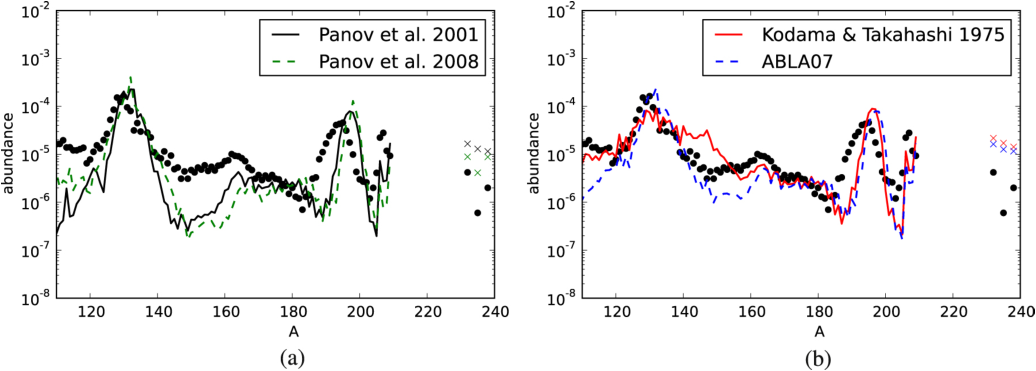
\includegraphics[width=0.9\linewidth]{TeX_files/rProc_abundances}
	\caption[Final r-process abundances for a neutron star merger scenario with different fission fragment distributions.]{Quoting their caption: "Final abundances of the integrated ejecta around the second and third peak for an NSM (Korobkin et al. 2012; Rosswog et al. 2013) at a simulation time $t={10}^{6}$ s, employing the FRDM mass model combined with four different fission fragment distribution models (see the text). For reasons of clarity the results are presented in two graphs. The abundances for Th and U are indicated by crosses. In the left-hand panel the lower crosses belong to the Panov et al. (2008) model (dashed line), while the lower crosses in the right-hand panel belong to the ABLA07 distribution model (dashed line). The dots represent the solar r-process abundance pattern (Sneden et al. 2008)." \cite{Eichler2015}}
	\label{fig:rprocabundances}
\end{figure}


Something interesting, and perhaps the kind of thing that might fit in with your thesis, is that there is a predicted four-hump pattern for the A=278 isobars in the SPY model (Scission Point Yield) \cite{Goriely2013}. This doesn't show up in the GEF, so far as I know, but it's interesting to think about. That could be an interesting thing to check a bit more carefully, since such a thing has never been observed experimentally. Also, 278Cf happens to be exactly halfway in between 266Cm and 290Fm. PS they actually show a PES for 278Cf in their Figure 3. I'm not 100\% convinced.

\section{Machine learning for r-process inputs}\label{sect:ml4rprocess}
Something that could be pretty doable and also moderately useful would be to use machine learning for fission yields to use in r-process network calculations. I got this idea from a guy at LLNL who gave a CMSE colloquium. He described a machine learning paradigm (he called it an ``Elevated Model'') in which they teach a deep learning network everything it could possibly care to know about a particular model - essentially, creating an emulator of the model. Then you kind of snip off the last couple of layers of your network, and reteach it (holding all but those last two layers constant), this time using experimental data. So by now you've gotten most of the physics intuition built into your emulator through the model training, and then for the physical insight your model misses (and perhaps to help reduce overfitting), you've taught it where the emulator goes wrong and what to do about it.

How can this help us fission folks? Well, right now the r-process network folks in the FIRE collaboration are using the GEF model for fission fragments and whatnot. It's basically a black box of magic that is super-overfitted and no one is completely sure how it works. BUT it's the best they've got for fission yields all across the region of interest, so that's what they use. My thought is to take this as a starting point (our ``model data''), and then use a combination of DFT calculations and also \textit{actual} experimental data as our experimental data. This could be an interesting opportunity to utilize your 290Fm results, along with anything else you've worked on.

Samuel worries (and I think, with justification) that we might not see any substantial improvements because the GEF is already so heavily overfitted. That, and that it might take a really long time (Leo's concerns are similar, plus he is concerned about having enough training data to do anything meaningful). That is why I'm thinking through what would need to be done, step by step, just to get a feel for a timeline of feasibility:
\begin{itemize}
	\item Finish a 290Fm calculation, just to have at least \textit{something} out there
	\item Figure out how to build a neural network where you can keep some layers fixed while selectively modifying others. I don't think that's something you could do in Scikit-learn; that you'd probably have to build custom (though fortunately you've already got something that might work!). Or you might be able to use TensorFlow (or Keras)
	\item Determine what observables you'd like (and are able) to include in your evaluation. For sure the locations of the peaks. Maybe also the width? Can you predict a full distribution from the same NN, or do you have to create a different one for each?
	\item Run the GEF for as many nuclei as you want to include in your evaluation
	\item Collect theoretical+experimental data you'll use to train your improved model
	\item Set aside a training set (Ideally you should include something that GEF clearly gets wrong compared to experiment, if possible)
\end{itemize}

The nice thing about this idea is that it can easily be extended or improved. Maybe some day Peter Moller has calculations across the landscape. You could just swap out the GEF data for Peter Moller's. Basically, it's just glorified interpolation, taking advantage of cheap models and combining/folding those with the more expensive, but more sparse, DFT and experimental results.

However, just based on Figure 1 of \cite{Vassh2018} and the preliminary yields I have for 266Cm and 290Fm, it doesn't look like we'd be adding too much new information. It looks to me like they already got the basic shape of the yields, and I don't know if I'd do much better with the localization fragment ID approach I'd been considering using. There is, however, a nice chart at the very end that shows candidate nuclei that are probably really important for their impact on final abundances, both in neutron-induced and beta-delayed fission. 290Fm doesn't seem to really fit but 266Cm isn't too far off.

\begin{figure}
	\centering
	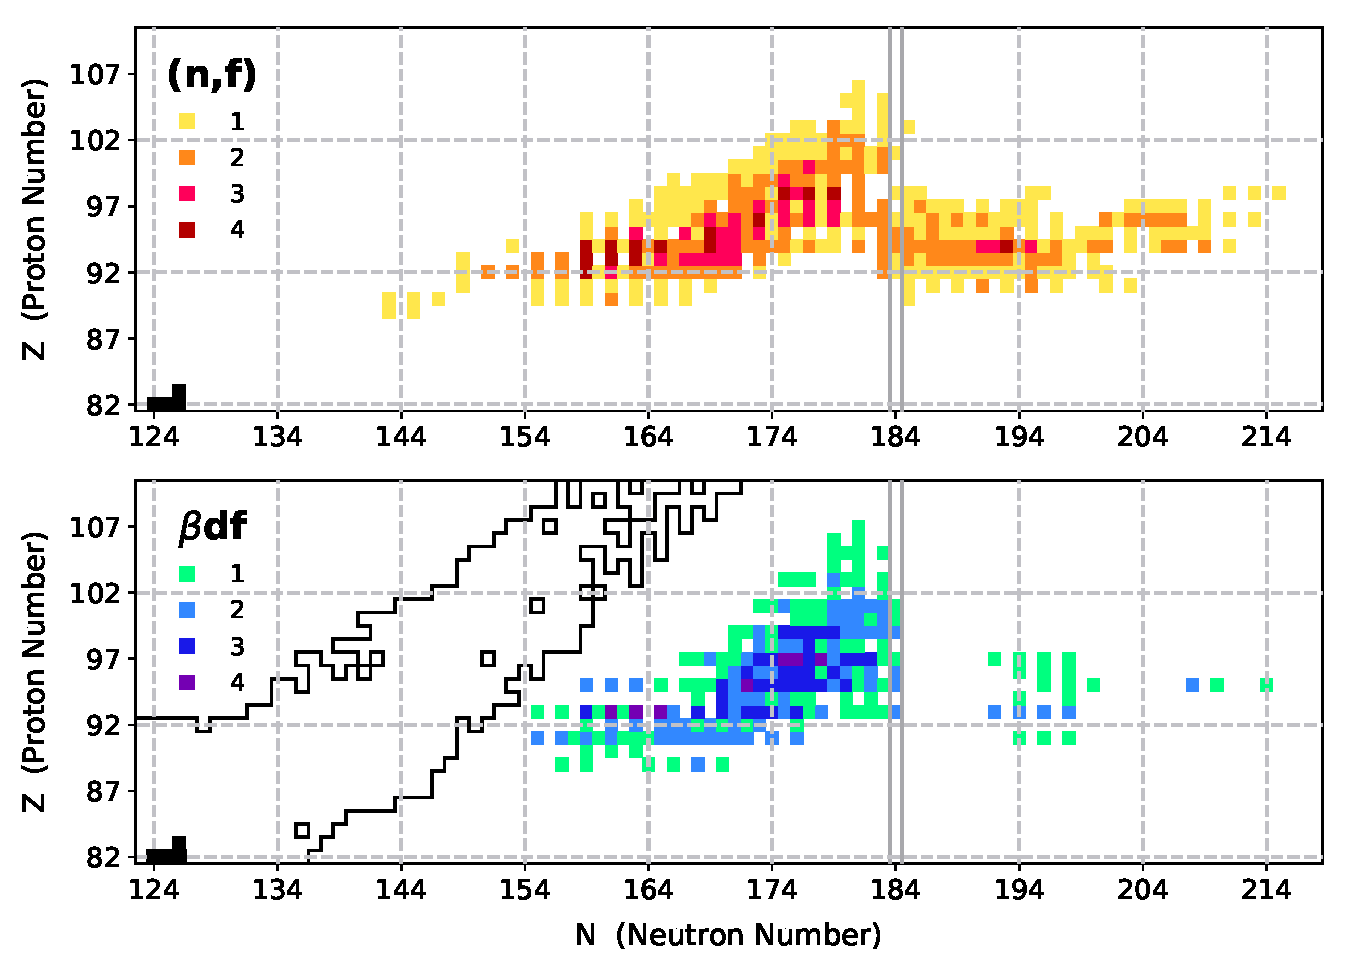
\includegraphics[width=0.7\linewidth]{TeX_files/rProc_important-fissions}
	\caption[Isotopes whose fission yields are especially relevant to the r-process]{Heatmap showing isotopes whose fission yields are especially relevant to the r-process. This combines the results from four different mass models, and counts how many mass models found each isotope to be relevant (integrated fission flow above a certain threshold). \cite{Vassh2018}}
	\label{fig:rprocimportant-fissions}
\end{figure}
